\documentclass[tikz,border=1pt]{standalone}
\begin{document}
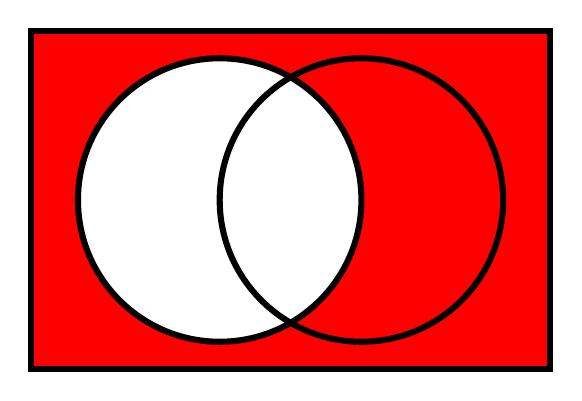
\begin{tikzpicture}
  \coordinate (A) at (-0.9,0);
  \coordinate (B) at (0.9,0);
  \def\r{1.8}
  \fill[red] (-3.3,-2.15) rectangle (3.3,2.15);
  \fill[white] (A) circle (\r);
  \draw[line width=2.2pt] (-3.3,-2.15) rectangle (3.3,2.15);
  \draw[line width=2.2pt] (A) circle (\r);
  \draw[line width=2.2pt] (B) circle (\r);
\end{tikzpicture}
\end{document}
